
\section{Applications existantes}

Aujourd'hui, il existe de nombreuses applications pour la recherche de restaurants : Yelp, Foursquare, Zomato, TripAdvisor et CROUS Mobile. Chaque application a sa propre particularité. \\

\bf{Yelp} est un site où sont répertoriés tous les avis des commerces locaux (alimentation, restaurant, shopping). Ce site est principalement actif dans les grandes villes.

\begin{figure}[H]
    \label{fig-yelp}
    \noindent\makebox[\textwidth]{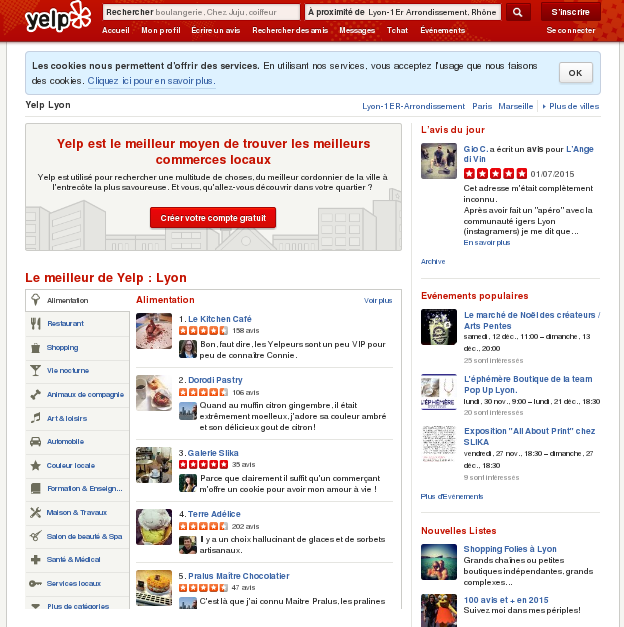
\includegraphics[width=10cm]{figures/yelp.png}}
    \caption{Capture d'écran de l'application Yelp}
\end{figure}

\bf{Foursquare} est un média social qui grâce à la géolocalisation permet d'indiquer à l'utilisateur  où il se trouve par rapport aux lieux d'intérêt (restaurants, cafés, magasins).

\begin{figure}[H]
    \label{fig-foursquare}
    \noindent\makebox[\textwidth]{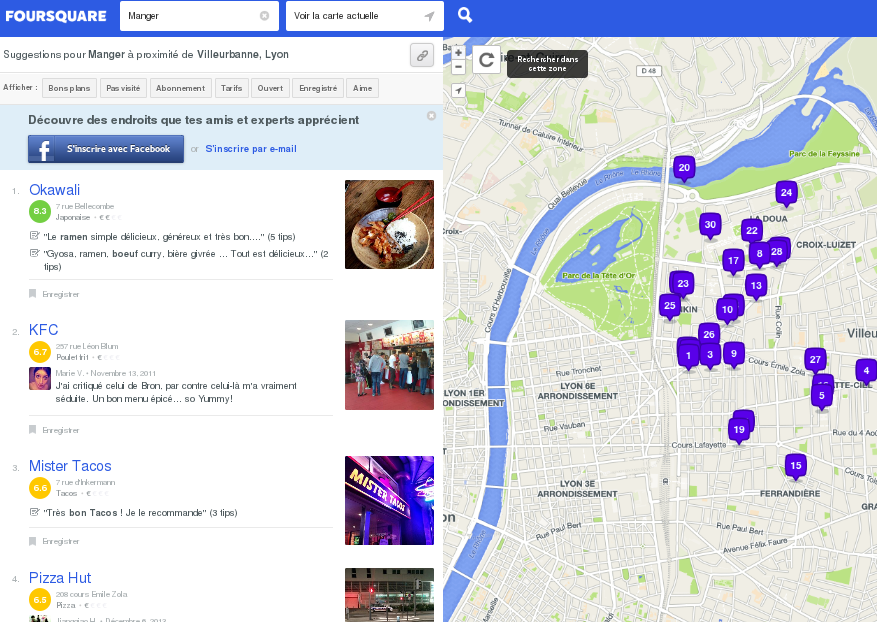
\includegraphics[width=10cm]{figures/foursquare.png}}
    \caption{Capture d'écran de l'application Foursquare}
\end{figure}

\bf{Zomato} est un annuaire des restaurants permettant de rechercher des informations sur les restaurants du monde entier (avis, photos). Il fonctionne sous la forme d'un réseau social où les utilisateurs publient des commentaires et des photos sur les restaurants et cela passe dans un fil d'actualité.

\begin{figure}[H]
    \label{fig-zomato}
    \noindent\makebox[\textwidth]{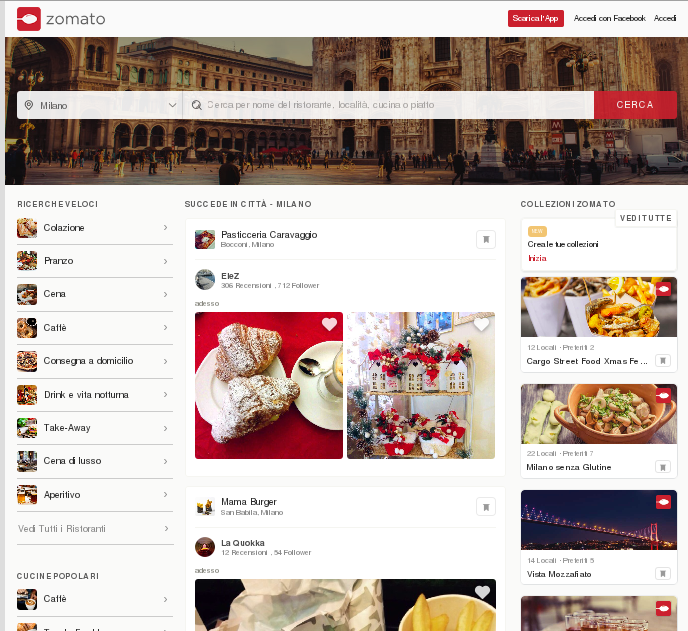
\includegraphics[width=10cm]{figures/zomato.png}}
    \caption{Capture d'écran de l'application Zomato}
\end{figure}

\bf{TripAdvisor} est un site web qui offre des avis et des conseils touristiques de consommateur (hôtels, restaurants, villes et régions, lieux de loisirs) et fournit également des outils de réservation de logements et de billets d'avion comparant des centaines de sites web afin de trouver les meilleurs prix.

\begin{figure}[H]
    \label{fig-trip-advisor}
    \noindent\makebox[\textwidth]{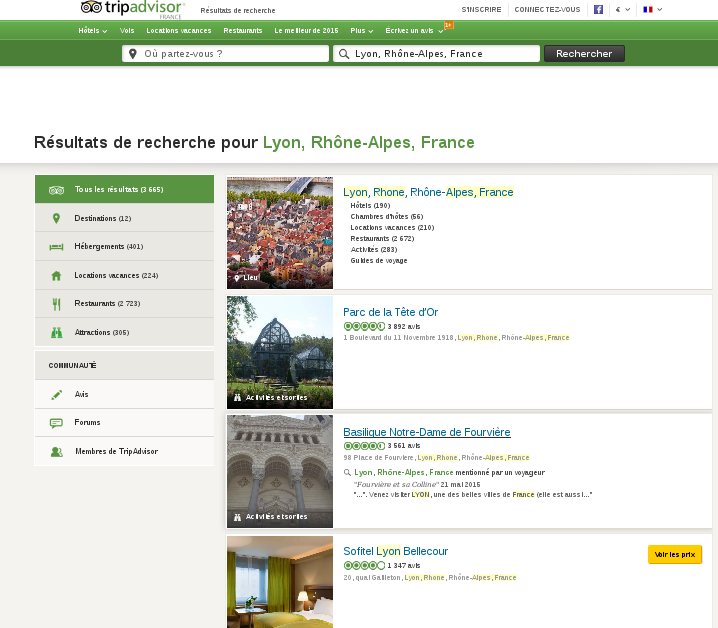
\includegraphics[width=10cm]{figures/trip_advisor.png}}
    \caption{Capture d'écran de l'application TripAdvisor}
\end{figure}

\bf{CROUS Mobile} est une application pour smartphone qui permet de retrouver toutes les informations du Crous (Restos U, logement, activités culturelles, services sociaux…).

\begin{figure}[H]
    \label{fig-crous-mobile}
    \noindent\makebox[\textwidth]{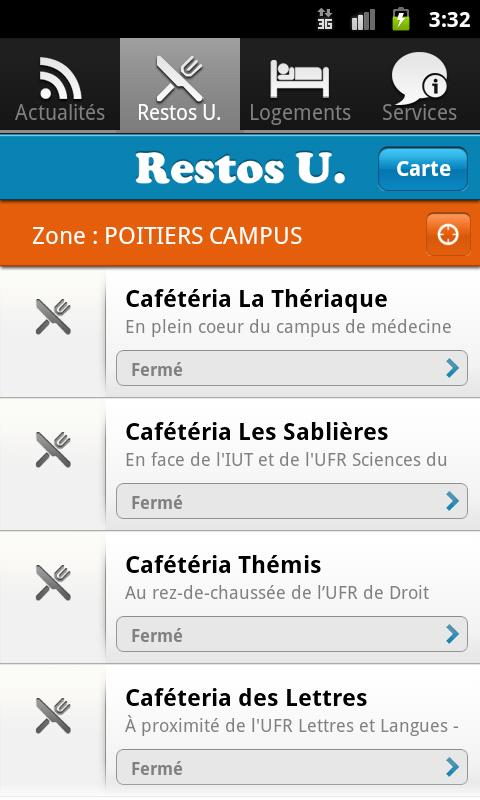
\includegraphics[width=6cm]{figures/crous_mobile.jpg}}
    \caption{Capture d'écran de l'application CROUS Mobile}
\end{figure}

\section{Conclusion}

Toutes ces applications sont destinées au grand public et ne répondent pas précisément au besoin 
exprimé par les utilisateurs à la suite de notre sondage. L'application que nous souhaitons développer cible, en effet, les étudiants et il s'agit là d'une niche. Les étudiants ne représentent pas une part très importante de la population mais il y aura toujours des étudiant. Il s'agit donc d'une niche dont l'existence est garantie et durable. Nous pouvons donc toujours envisager de développer cette application sans craindre d'avoir à nous insérer dans un marché déjà occupé par d'éventuels concurrents.
